%!TEX root = ../main.tex
\section{Background of Coreset Selection} 
\label{sec:pre}

In this section, we introduce the background of coreset selection on complete data, denoted by $\trainc$.
%, based on which we  illustrate the framework of  selecting the coreset over the incomplete data.

\subsection{Gradient Descent for Machine Learning}

{\bf Gradient descent}~\cite{lemarechal2012cauchy} is the most typical optimization algorithm to train ML models. 
At a high level, it  tweaks the parameters iteratively to minimize a given convex and differentiable function to its local minimum.

Let $\trainc = \{t_1, t_2, ..., t_n \}$ be a set of train tuples (without missing values), where $t_i = (\mathbf{x}_i, \mathbf{y}_i)$, $\mathbf{x}_i \in \mathbb{R}^d$ denotes the vector of features and $\mathbf{y}_i$ denotes the corresponding label. The goal of training on $\trainc$ is to find the best parameter  $\hypo^*$ of an model by minimizing the loss:

\vspace{-0.5em}
\begin{equation}\label{eqa:loss}
\hypo^* = \arg\min_{\hypo\in \vartheta}\fun(\hypo), \fun(\hypo)=\frac{1}{n}\sum_{i=1}^n\fun_i (\hypo, t_i) 
\end{equation}

\noindent where $\vartheta$ is the parameter space. For ease of representation, we abbreviate $\fun_i (\hypo, t_i)$ as $\fun_i(\hypo)$ to represent the loss of the $i$-th train example.  Generally speaking, the gradient descent approach is always applied to find the minimizer of  Eq.~\ref{eqa:loss}, where  the {\bf full gradient} (sum of the gradients over all training tuples), denoted by $\nabla\fun(\hypo) = \sum_{i=1}^{n}\nabla\fun_i(\hypo)$, has to be computed iteratively. 

Besides incremental gradient methods like stochastic gradient descent (SGD) that can be leveraged to accelerate the iterative gradient computation, there are other popular and orthogonal methods, such as coreset, which will be discussed next.

%it is still expensive when there are a large number of train tuples.


\subsection{Coreset over Complete Data}
\label{subset:sigletable}

\stitle{Coreset.} To make training more efficient, instead of learning from entire $\trainc$, one research question  is that whether we can compute a small subset $\corefunc(\trainc)$ of $\trainc$ such that learning with $\corefunc(\trainc)$ can hopefully achieve the same performance as learning with $\trainc$.
%
This small selected subset is called {\bf coreset}~\cite{DBLP:journals/corr/abs-2011-09384,munteanu2018coresets}.
%
In the following, we simply write $\corefunc(\trainc)$ as $\core$ when it is clear from the context.

The state-of-the-art coreset selection solutions are mostly based on gradient approximation~\cite{DBLP:conf/aaai/KillamsettySRI21, DBLP:conf/icml/MirzasoleimanBL20}.
Suppose that $\theta$ denotes the parameter of an ML model trained over the full dataset, and $\theta'$ denotes the parameter of the same model trained over  the coreset.   Intuitively,   the objective of gradient approximation for coreset selection is to make $\nabla\fun(\hypo')$ as close as possible to $\nabla\fun(\hypo)$. To this end, existing solutions focus on \textit{selecting the coreset that  minimizes the upper bound of gradient approximation error} ($\lVert  \nabla\fun(\hypo) - \nabla\fun(\hypo')  \rVert$). Next, let's formally define it from scratch.
%


%Based on gradient approximation, existing solutions can lead to good performance with theoretical guarantees, \ie $\nabla\fun(\hypo)$ is upper-bounded by $\nabla\fun(\hypo')$. Next let's formally define it.

%Given a large training dataset $\train$, in general,  coreset selection in ML aims to compute a small subset $\core$ of $\train$ such that training on  $\core$ can hopefully has the same performance as training on $\train$, which is inefficient due to the large amount of data.  Although there exist a line of approaches, coreset selection considering the gradient approximation is a commonly-used one because of the good performance with theoretical guarantees. 


%\subsection{Problem definition}  \label{subsec:def}

%In this section, we first introduce the  definition of coreset in the field of ML, and then formally define our problem of coreset selection over multiple tables.

%\subsubsection{Coreset selection over a single table}\label{subsubsec:singleTab}  Given a large training dataset $\train$, in general,  coreset selection in ML aims to compute a small subset $\core$ of $\train$ such that training on  $\core$ can hopefully has the same performance as training on $\train$, which is inefficient due to the large amount of data.  Although there exist a line of approaches, coreset selection considering the gradient approximation is a commonly-used one because of the good performance with theoretical guarantees. 

% \noindent \textbf{Training on $\train$.}  Formally speaking, $\train = \{t_1, t_2, ..., t_n \}$ is a set of labeled training tuples, where $t_i = (\mathbf{x}_i, \mathbf{y}_i)$, $\mathbf{x}_i \in \mathbb{R}^d$ denotes the feature vector and $\mathbf{y}_i$ is the corresponding labels.
% The objective of training on $\train$ is to compute the best parameter  $\hypo^*$ to minimize the loss


% \begin{equation}\label{eqa:loss}
%     \fun(\hypo)=\frac{1}{n}\sum_{i=1}^n\fun_i (\hypo, t_i), \hypo^* = \arg\min_{\hypo\in \vartheta}\fun(\hypo)
% \end{equation}

% \noindent where $\vartheta$ denotes the parameter space and for ease of representation, we just use $\fun_i(\hypo)$ to denote the loss of the $i$-th training example, \ie $\fun_i (\hypo, t_i)$.  Typically, the gradient descent method is always applied to optimize Eq.~\ref{eqa:loss}, where  the full gradient, \ie $\nabla\fun(\hypo)$ is required to compute iteratively. Although some classic incremental gradient methods such as  stochastic gradient descent (SGD), can be utilized to accelerate this process, it is still expensive when there are massive training tuples.



\stitle{Gradient-based coreset selection} %To alleviate the above issue, coreset is proposed to  
%It is to select a subset $\core\subseteq \train$ such that the sum of weighted gradients of tuples in $\core$ can well approximate the full gradient $\sum_{i=1}^{n}\nabla\fun_i(\hypo)$. The goal is, training on $\core$ based on the estimated gradient is very likely to achieve the same performance as training on the entire training set. Formally, it is defined as follows:
%Let $\nabla\fun(\hypo) = \sum_{i=1}^{n}\nabla\fun_i(\hypo)$ be the full gradient training using the entire train dataset, the problem of coreset selection 
is to minimize the {\bf gradient approximation error (GA error)} between the full gradient \wrt $\trainc$ and the weighted sum of gradients \wrt the coreset $C$ (or coreset gradient).
Formally, Eq.~\ref{eqa:coreset} tries to minimize the  GA error 
by considering all possible parameters $\hypo\in\vartheta$ (\ie $\max\limits_{\hypo\in\vartheta}$), where ``$\| \cdot \|$'' denotes the normed difference. Next, we introduce the coreset gradient.
%in details.

\vspace{-1em}
\begin{equation}\label{eqa:coreset}
\begin{array}{l}
\core^* = \argmin\limits_{C\subseteq \trainc, w_j \geq 0}
\max\limits_{\hypo\in\vartheta}
\lVert 
\underbrace{
	\underbrace{\sum\limits_{i=1}^n\df_i(\hypo)}_{\text{full gradient}} - 
	\underbrace{\sum\limits_{j=1}^{|C|}w_j\df_{\gamma(j)}(\hypo)}_{\text{coreset gradient}} 
}_{\textbf{gradient approximation error}}
\rVert, 
\\ 
s.t.~|C| \le \numcore %\le \epsilon
\end{array}
\end{equation}




%The {\bf full gradient} has been defined earlier as $\nabla\fun(\hypo) = \sum_{i=1}^{n}\nabla\fun_i(\hypo)$.Next, let's focus on explaining how to compute the {\bf coreset gradient} in Eq.~\ref{eqa:coreset}.
%
%\noindent since  $\core\subseteq \train$ with the size no more than $K$,
Because the coreset is a subset of the complete dataset (\ie $C \subseteq \trainc$),
we use $\gamma(j) = i$ (where $j\in[1,|C|], i\in[1,n]$) to denote that the $j$-th tuple in $\core$ (denoted by $c_j$) is the $i$-th tuple in $\trainc$, \ie $t_i$. In other words, $\gamma$ is an index mapping from $\core$ to $\trainc$. 

Recall that the key idea of the coreset is to \textit{use a subset of tuples to represent the entire set}.  Eq.~\ref{eqa:coreset} potentially contains another important mapping $\phi$ from $\trainc$ to $\core$ to indicate this, \ie $\phi(i) = j, i\in[1,n],  j\in[1,|C|]$, which is highly related to the weight. Specifically, let $\phi(i) = j$ denote that we will assign  $t_i$ to $c_j$ (use $c_j$ to represent $t_i$) and use $\df_{\gamma(j)}$  to represent $\df_i$. Each $t_i$ will be assigned to one and only one $c_j$, but each  $c_j$ might be assigned with multiple tuples in $\trainc$. Based on $\phi$,
$w_j$ is defined as the weight of  the $c_j$, which is the number of tuples in $\trainc$ assigned to the $c_j$, \ie $w_j = |\{t_i|\phi(i) = j, i\in[1,n]\}|$ ($c_j$ is utilized to represent $w_j$ tuples in $\trainc$). 

Next let's use an example to better illustrate Eq.~\ref{eqa:coreset}.



\begin{example}\label{example:singletable}
	Let's consider a  case of the gradients of each tuple, as shown in Figure~\ref{fig:overviewSingle}. Suppose that for any $\hypo$, $\df_1(\hypo)\approx\df_2(\hypo)$, $\df_3(\hypo)\approx\df_4(\hypo)\approx\df_5(\hypo)\approx\df_6(\hypo)$ and $\df_7(\hypo)\approx\df_8(\hypo)$. In this case, based on Eq.~\ref{eqa:coreset}, if one wants to find an optimal coreset with a size of  3, \ie $\numcore=3$, the solution can be $C^* = \{t_2, t_5, t_7\}$ ($\gamma(1)=2, \gamma(2)=5$ and $\gamma(3)=7$), associated with $w_1=2, w_2=4, w_3=2$ because $\phi(1) = \phi(2) = 1, \phi(3) = \phi(4) = \phi(5) = \phi(6) = 2 $ and $\phi(7) = \phi(8) = 3$. In this way, $C^*$ can be one of the optimal coresets that can well approximate the full gradient because  $\lVert \sum\limits_{i=1}^8\df_i(\hypo) - \sum\limits_{j=1}^{3}w_j\df_{\gamma(j)}(\hypo) \rVert  $ is minimized, which is close to 0.
\end{example}


\begin{figure}[t]
	\centering
	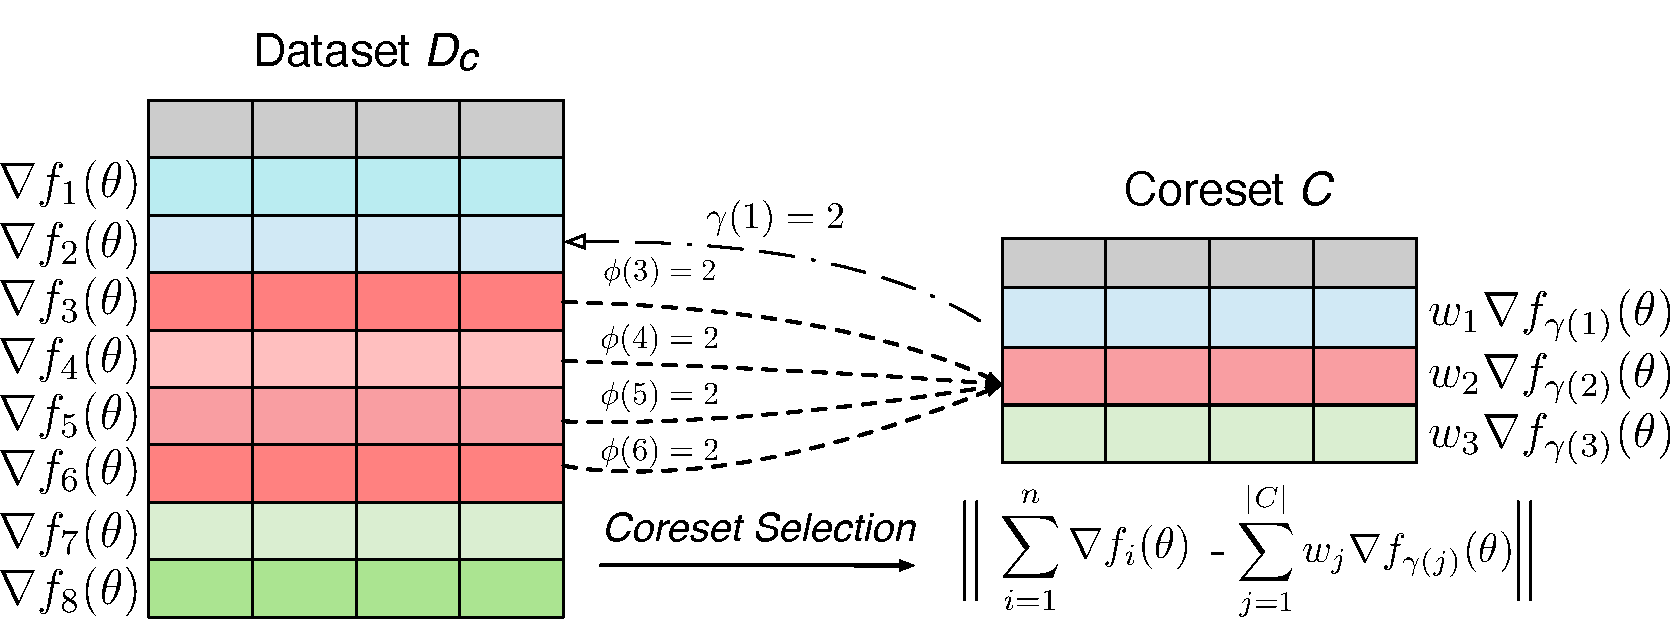
\includegraphics[width=0.6\textwidth]{figs/coresetExample}
%	\vspace{-2em}
	\caption{Example of coreset selection.}
	\label{fig:overviewSingle}
%	\vspace{-2em}
\end{figure}

\stitle{Key observation.} We can observe from Example~\ref{example:singletable} that in order to minimize the GA error, we should set $\phi(i) = j$, where $\df_i$ and $\df_{\gamma(j)}$ are likely to be close. 
Therefore, computing the coreset is similar to computing the $\numcore$ exemplars~\cite{rdusseeun1987clustering} of the gradients, if all the gradients of tuples can be computed.


\stitle{Upper bound minimization of GA error.} We can see from Eq.~\ref{eqa:coreset} that to solve the equation, the gradients have to be computed, which have a close relationship with the parameter  $\theta$. However, the main bottleneck is that  the entire parameter space $\vartheta$ is too expensive to explore. Hence, a typical solution is to  first compute the upper bound of  GA error (Eq.~\ref{eqa:triangle}),  then generalize~\cite{hofmann2015variance, allen2016exploiting,DBLP:conf/icml/MirzasoleimanBL20} the upper bound computation to the entire parameter space (Eq.~\ref{equation:convex}), and finally select the coreset to minimize the bound. To be specific, using the triangle equation, for any particular $\theta$, we have:

\vspace{-0.5em}
\begin{equation}\label{eqa:triangle}\small
\begin{array}{l}
\lVert 
\sum\limits_{i=1}^n\df_i(\hypo) - 
\sum\limits_{j=1}^{|C|}w_j\df_{\gamma(j)}(\hypo) 
\rVert \leq \sum\limits_{i=1}^n \lVert \df_i(\hypo) - \df_{\gamma(\phi_\theta(i))}(\hypo) \rVert
\end{array}
\end{equation}

Together with the aforementioned observation, given a coreset $\core$, the upper bound is minimized when  $\phi$ assigns
every tuple $t_i$ to the tuple in $\core$ with most gradient similarity, \ie $\lVert 
\sum\limits_{i=1}^n\df_i(\hypo) - 
\sum\limits_{j=1}^{|C|}w_j\df_{\gamma(j)}(\hypo) 
\rVert \leq \sum\limits_{i=1}^n \min \limits_{c_j\in\core}\lVert \df_i(\hypo) - \df_{\gamma(j)}(\hypo) \rVert$.

\stitle{For the entire space $\vartheta$},  it has been proved in recent works~\cite{hofmann2015variance, allen2016exploiting,DBLP:conf/icml/MirzasoleimanBL20} that for convex ML problems (corresponding to an optimization problem in which the objective function is a convex function), the normed gradient difference between tuples can be efficiently bounded by:

\vspace{-0.5em}
\begin{equation}\label{equation:convex}
\begin{aligned}
\forall  i, j, \max\limits_{\hypo\in\vartheta}\lVert \df_i(\hypo) - \df_j(\hypo) \rVert \le \max\limits_{\hypo\in\vartheta}\mathcal{O}(\lVert \theta \rVert) \cdot \lVert \mathbf{x}_i - \mathbf{x}_j \rVert
\end{aligned}
\end{equation}

\noindent where $\lVert \mathbf{x}_i - \mathbf{x}_j \rVert$ is the Euclidean distance between  feature vectors of two tuples, namely \textit{feature distance}, and 
 $\mathcal{O}(\lVert \theta \rVert)$ is a constant. Hence, we can conclude that \textbf{GA error can be bounded independent of the optimization problem in practice, \ie any particular $\theta$}. Finally, considering Eq.~\ref{eqa:triangle} and  Eq.~\ref{equation:convex} together,  \textit{the coreset selection problem can be converted to:}
 
 \vspace{-0.5em}
 \begin{equation}\label{eqa:coreset2}
 \core^* = \argmin\limits_{C\subseteq \trainc}\sum_{i=1}^n \min_{c_j\in C}\dist_{ij}, \text{ s.t. } |C| \le \numcore %\le \epsilon
 \end{equation}
 
 \noindent where $\dist_{ij} = \lVert
 \mathbf{x}_i - \mathbf{x}_{\gamma(j)}  \rVert$ for ease of representation. The above equation indicates that given a train data $\trainc$ and a coreset $\core$, we use  $S = \sum_{i=1}^n \min_{c_j\in C}\dist_{ij}$ to score the coreset. The lower the score, the smaller upper bound of the GA error we can get, which indicates a better coreset.
 To summarize, solving Eq.~\ref{eqa:coreset2} is to minimize the upper bound of the GA error (\ie select the coreset with the lowest score) by just considering the feature vectors of the training tuples without  training in advance.
 
Note that Eq.~\ref{equation:convex} holds for tuples associated with the same label~\cite{allen2016exploiting, hofmann2015variance}. Therefore, in practice, we respectively select coresets for tuples with different labels and combine them. Suppose that we aim to select a coreset with size  $K$ for a binary classification task (label 1: 60\%, label 0: 40\%), so we select a coreset with size 60\%$K$ for tuples with label 1 and another one with 40\%$K$ for tuples with label 0.
%we need to select subsets of coresets for tuples with dierent labels
%and combine them. For example, given a binary classication task
%(30\% of label 0 and 70\% with label 1), to select a coreset with size $K$,
%we separately select a coreset of size 30\%$K$ for tuples with label 0
%and another coreset of size 70\%$K$ for tuples with label 1, and then
%merge them. For regression tasks, we will cluster tuples with similar labels, select subsets of coresets for these clusters and merge them.
 
\stitle{Our scope.} In this paper, we focus on the convex problems (\eg logistic regression, support vector machine, etc.) because for such
problems the gradient difference can be well bounded by the difference
between feature vectors. 
%
Note that, for other ML algorithms such as deep neural networks, they can also be trained using selected coreset to achieve good training accuracy (see Section~\ref{sec:exp} for our experimental findings).

% \cc{For other ML algorithms, like
% deep learning, can also train on the selected the coreset. As shown in Section~\ref{sec:exp}, good performance can also be achieved although it is hard to have a theoretical gradient bound.}

\section{Coreset Over Incomplete Data} % ($\train$)}
\label{sec:overview}

In this section, we will formally define the problem of coreset selection over incomplete data (Section~\ref{subsec:problem}) and then describe our proposed framework to solve the problem  (Section~\ref{subsec:framework}).

\subsection{Problem Definition}
\label{subsec:problem}



As discussed above, we have to compute the coreset score $S$, so as to produce a good coreset.  To this end, the feature distances can be computed as a pre-processing step, based on which the coreset score can be computed. However, when there exists incomplete data with missing values, even the feature distances are hard to compute accurately, let alone selecting a proper coreset.

\stitle{Incomplete data.}
Formally, suppose that $\train$ has $M$ attributes, denoted by $\{\attr_1, \attr_2, ..., \attr_M\}$. Each attribute $\attr_m, m\in [1,M]$ represents a  domain set including the \texttt{Null}, (\ie $\texttt{Null} \in \attr_m$), in which each tuple in $\train$ can take value on this attribute. $|\attr_m|$ denotes the domain size. Then, each tuple $t_i \in \attr_1 \times \attr_2 \times, ..., \times \attr_m$. Let $t_i[m]$ denote the value of the $m-$th attribute of $t_i$, \ie $t_i[m] \in \attr_m$.
 
 
 For a tuple $t_i\in \train$, if $\exists~ t_i[m] = \texttt{Null},m\in [1,M] $, $t_i$ is an incomplete tuple, denoted by $\mathbb{I}[t_i] = 1$, otherwise $\mathbb{I}[t_i] = 0$.
Let us better illustrate this using an example. 

\begin{example} \label{example:incomplete}
	As shown in  Figure~\ref{fig:missing}(a), there are 6 tuples in the table $\train$ with five attributes (an excerpt from a large table). For example, $\attr_2$ is the \texttt{Gender} attribute, \ie $\attr_2 = \{ \texttt{M}, \texttt{F}, \texttt{Null} \}$.
	 Among these tuples, $t_2, t_3, t_4, t_6$ have missing values, \eg $\mathbb{I}[t_2] = 1, \mathbb{I}[t_1] = 0$. Given a coreset as shown on the right side, if there are no missing values, we can assign each tuple $t_i\in \train$ to its most similar tuple in $\core$ (compute $\min_{c_j\in C}\dist_{ij}$), and then sum these feature distances up to  compute the coreset score  $S$. However, given these missing values, the feature distances cannot be computed accurately (\eg $s_{12}, s_{13}, s_{22}$, etc.), and thus the assignment of tuples in $\train$ cannot be determined precisely. Hence, the coreset score is not precise, and thereby leads to a  coreset that cannot well represent the full complete (clean) data. 
	 \vspace{-0.3em}
\end{example}


\begin{figure}[t]
	\centering
	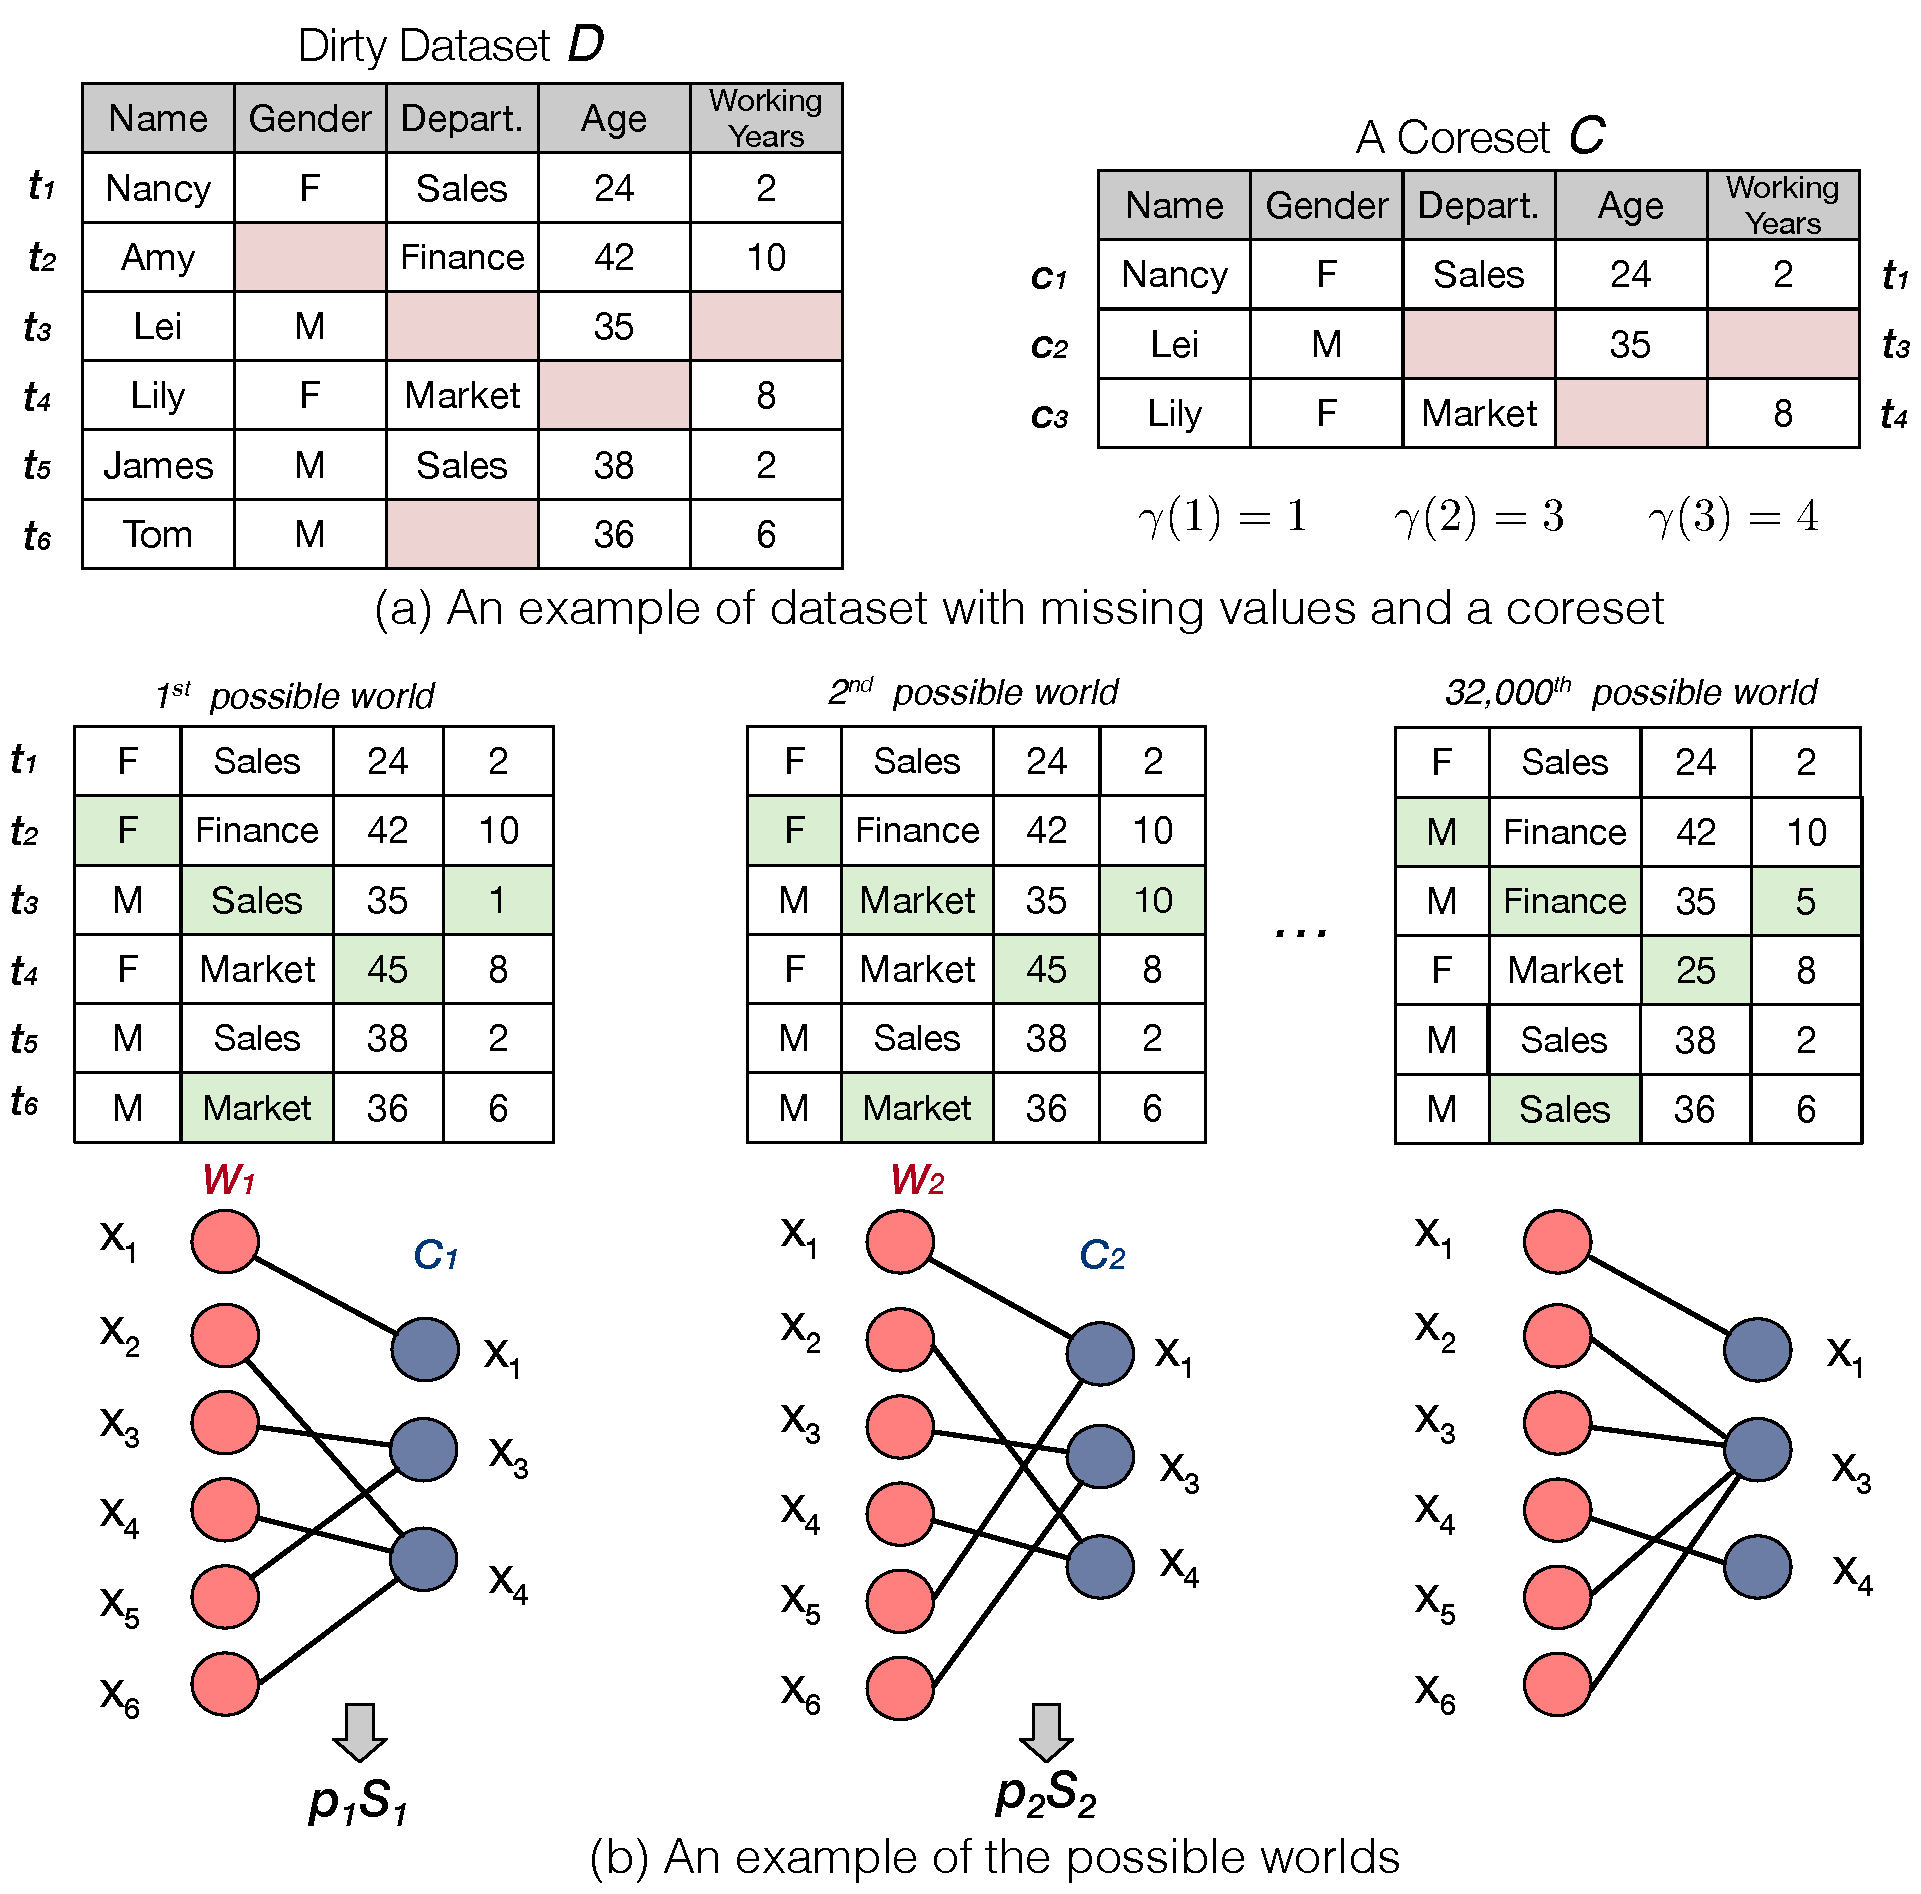
\includegraphics[width=0.6\textwidth]{figs/missExample}
%	\vspace{-2.5em}
	\caption{Example of coreset selection with missing values}.
	\label{fig:missing}
%	\vspace{-1.7em}
\end{figure}

As discussed above, \textit{imputation before coreset selection} suffers from either large cost (human imputation) or large number of possible repairs (automatic imputation), while \textit{imputation after coreset selection} cannot obtain a good coreset  because of the inaccurate feature distance computation (see Example~\ref{example:incomplete}).

%\etitle{Imputation before Coreset Selection.}
%One natural direction is to impute missing values before coreset selection. 
%As discussed in Section~\ref{sec:intro}, we can ask humans to impute the missing values first accurately and then select the coreset, but it is rather expensive given a large number of missing values, as discussed in Case (1) in Section~\ref{sec:intro}. 
%
%Alternatively, we can choose existing automatic imputation methods, as shown in Case (2).
%However, automatic  methods typically cannot ensure high imputation accuracy because these missing values result in a large number of possible repairs, which constitute a large search space. Therefore, it is hard for  automatic methods to identify an accurate imputation, based on which the selected coreset is also not good enough.
%the  they are not always accurate because these missing values result in a large number of possible worlds, and then produce a very large search space. 

%\etitle{Imputation after Coreset Selection.} Instead, we can select the coreset first, and then leverage human or automatic methods to impute the coreset, as illustrated in Case (3) and (4). However, the coreset directly selected from  incomplete data $\train$ is not good enough because of the inaccurate feature distance computation (see Example~\ref{example:incomplete}), and thus although humans can provide accurate imputation with a low cost, it is also hard for the coreset to well represent  $\trainc$.

Therefore, an essential problem is to select a good coreset that can represent the complete dataset $\trainc$, which relies on accurate coreset score computation given $\trainc$ that is the unknown ground truth.
%
Fortunately, the possible repairs of $\train$ can be modeled by possible worlds~\cite{DBLP:journals/tods/DengFG16, DBLP:conf/pods/ArenasBC99, DBLP:series/synthesis/2011Bertossi, DBLP:conf/pods/Bertossi19}, based on which we can effectively select the coreset over incomplete data.

%\cc{In short, the key is to select a good coreset that can represent $\trainc$, which relies on accurate coreset score computation given $\trainc$ and a coreset, but unfortunately $\trainc$ is the ground truth unknown in advance, 
%	To alleviate this issue, we can model possible repairs of $\train$ such that the selected coreset can represent the expected situation of $\trainc$.
%To this end, we leverage the  possible worlds that are widely-used in data repairing~\cite{DBLP:journals/tods/DengFG16, DBLP:conf/pods/ArenasBC99, DBLP:series/synthesis/2011Bertossi, DBLP:conf/pods/Bertossi19} to select the coreset over incomplete data.}


%Next, we first formally define the possible worlds.

%\begin{definition}(Possible worlds) 
\stitle{Possible worlds.}
 Given   the incomplete dataset $\train$, $\forall t \in \train$ and $\mathbb{I}[t] = 1$, $ \forall t[m] = \texttt{Null}, m \in[1, M]$, we assign a value in $\attr_m\setminus \{ \texttt{Null}\}$ to $t[m]$ as an imputation (\aka a possible repair). Thus, we have an assignment for all the missing values in $\train$, which corresponds to a possible world $\world$. Since there exist a large number of possible assignments,
 we define the set of possible worlds as $\worlds=\{\world_k| k\in [1,|\worlds|] \}$.
 %\end{definition}
 
 Let us better illustrate this using an example.
	

\begin{example}
	
Given $\train$, for tuples $t_2, t_3, t_4, t_6$ with missing values, we have a large number of possible assignment  as shown in Figure.~\ref{fig:missing}(b), each of which corresponds to a possible world (we omit the \texttt{Name} attribute because there is no missing value on this attribute). Suppose that there are 2 (4/100/10) types of values of the attribute \texttt{Gender} (\texttt{Department}/\texttt{Age}/\texttt{Working years}), there exist 32,000 possible worlds in total. %\cc{
	%}
\vspace{-0.3em}
\end{example}

Note that for numerical attributes, we will bin them into different buckets, such that we can treat them as categorical values and avoid the unlimited number of possible worlds.

Even with  possible worlds, the score computation of coreset remains challenging. 
Each possible world of $\train$ is a complete dataset, and thus given a coreset, the score can be directly computed considering the feature distances, as discussed in Section~\ref{subset:sigletable}. However, the crucial issue is that each possible world could be the ground truth, \ie $\trainc$, but each one leads to a different score.
%
%\nan{Only saying ``the score can be much different'' is not strong enough for the challenge. We need to use more conceptual idea here. \textbf{Why hard when using possible words?}}

\begin{example}
\label{exam:diffscores}
	As shown in Figure.~\ref{fig:missing}(b), the two possible worlds $\world_1$ and $\world_2$ are only different in $t_3$, leading to a different feature vector $\mathbf{x}_3$, which makes the score computation a difference. To be specific, given the same coreset $\core$ with tuples $t_1 (c_1)$, $t_3 (c_2)$ and $t_4 (c_3)$, because of a different $\mathbf{x}_3$, the closest feature distance of $\mathbf{x}_5$ in $\world_2$ becomes $\mathbf{x}_1$, rather than $\mathbf{x}_3$ in $\world_1$. And the closest feature distance of $\mathbf{x}_6$ in $\world_2$ becomes $\mathbf{x}_3$, rather than $\mathbf{x}_4$ in $\world_1$. Therefore, the coreset scores, %($S=\sum_{i=1}^n \min_{c_j\in C}\dist_{ij}$), 
	\ie the sum of these closest feature distances of tuples are different among possible worlds.
	\vspace{-0.3em}
\end{example}

Example~\ref{exam:diffscores} shows that different possible worlds make the mapping $\phi$ different, which leads to different scores. Hence, to get a good coreset without the ground truth, an intuitive solution is to compute the expected coreset score considering all possible worlds. By doing so, although we cannot get the complete data ($\trainc$) in advance, we can focus on how to select an informative coreset that can represent the possible worlds of $\train$.

Next, we formally define the studied problem.

%\begin{definition}[Expected optimal coreset selection over incomplete data]
\stitle{Expected optimal coreset selection over incomplete data.}
	 %Given $\train$ and $\core$, we have possible worlds $\{W_k\}$ as well as the corresponding coresets $\{C_k\}$. 
	 Given $\train$, we have a number of possible worlds $\worlds=\{W_k\}$. Then given a subset (coreset) $C\subset \train$,  
	  for different $W_k$, we have the corresponding $C_k$ with the same tuples as $C$ but probably different imputations.
	   For $C_k$, we can compute a score $S_k = \sum_{i=1}^n \min_{c_j\in C_k}\dist_{ij}$, where $\dist_{ij} =  \lVert\mathbf{x}_i - \mathbf{x}_{\gamma(j)}\rVert$ and   both feature vectors are from $\{W_k\}$. Then, we have the expectation $\mathrm{E}[C] = \sum_{k= 1}^{|\worlds|} p_kS_k$, where $p_k$ denotes the probability of the appearance of  $\{W_k\}$.
	Finally, our problem becomes how to compute the coreset $C$ with the lowest expectation of GA error upper-bound. Formally, we have
	\begin{equation}\label{eqa:expectation}
	\core^* = \argmin   \limits_{C\subseteq \train}\mathrm{E}[C], \text{ s.t. } |C| \le \numcore %\le \epsilon
	\end{equation} 
%\end{definition}

%\cc{
For example, given $\train$, the corresponding possible worlds and a coreset $C$ in Figure~\ref{fig:missing}, we have different $C_k$ with the same tuples (containing $t_1, t_3, t_4$) but probably different imputations. For each $C_k$, we will compute $S_k$, and finally compute $\mathrm{E}[C]$. Solving Eq.~\ref{eqa:expectation} can result in an informative coreset with incomplete tuples being selected. After these tuples imputed by a human, \ie Case (5), or state-of-the-art automatic method, \ie Case (6), we can derive a good coreset.
%}

%Given a coreset $\core$, we can find that different possible worlds may have different coreset scores. For example, to compute an accurate coreset score, we consider the expected coreset score for each coreset, denoted by XX. Then, the problem becomes how to compute the optimal expected coreset with the lowest expectation score. Formally,







%To be specific,  given two tuples $x_i$ and $x_j$, if any tuple has missing values, the 	feature difference between them cannot be computed accurately. As discussed in Section~\ref{sec:intro}, we can leverage humans/oracle to accurately impute the missing data

%However, the data can be dirty in real world, for example, the missing values. In short, if every pair of $||x_i - x_j||$ can be computed accurately, the coreset is the correct one. Suppose $x_i'$ is a dirty data instance with a missing attribute $a$ (corresponding to the clean one $x_i$), and thus the $\forall j \in S, d_{ij}$ should be computed by $\texttt{const} \cdot ||x_i' - x_j||$, which is not accurate.

%Although  $x_i'$ is a dirty instance, only few attributes of $x_i'$ is dirty.  For each missing attribute of the dirty instance,  \textit{ the missing values  have several candidates to be filled}. Suppose that for $x_i'$ with three possible values of the attribute $a$, leading to $x_i^1, x_i^2, x_i^3$, and $x_i$ must be one of them. 








\iffalse

\noindent \textbf{Compute the expectation.}  In this part, we try to solve the Eq.~\ref{eqa:expectation}, which roughly consists of  two steps. One is to  select the a subset $\core$, and the other is to compute the expectation $\mathrm{E}[\sum_{i\in \train} \min_{j\in \core} d_{ij}]$ such that the smallest subset satisfying the constraint can be selected. In Eq.~\ref{eqa:core}, $\sum_{i\in \train} \min_{j\in \core} d_{ij}$ is easy to compute in linear time, but how about the expectation? To illustrate this, we have to show what is the expectation like, where the possible world is the key point.







\noindent \textbf{Possible world.} Given the full training dataset $\train$, we  can easily derive a dirty subset $\train' \subset \train$, where $\forall t\in \train'$ has at least one missing attribute. For ease of representation, we just consider the case that each data instance just has one missing value.  We assume that each missing attribute $t[a]$ has $k$ (which can be viewed as a constant) possible values, each of which is denoted by $t_i[a], i\in[1,k]$, and $p(t_i[a])$ represents the likelihood that the missing value $t[a]$ being $t_i[a]$.
Therefore, there are $O(k^{|\train'|})$ possible  assignments in total, each of which corresponds to a possible world. 

Let us better illustrate this using an example.



In general, we denote the sets of possible worlds as $\mathcal{P} = \{\mathbf{P}_1, \mathbf{P}_2, ..., \mathbf{P}_{|\mathcal{P}|}\}$, where each possible world $\mathbf{P}_i$ corresponds to a probability $p_i$.
$p_i$ can be directly computed by the multiplication of the probabilities of possible values, i.e., $p_i = \prod_{t\in \train'} p(t_j[a]), t_j[a] \in \mathbf{P}_i$.  
Given $\train,\core$,  different possible worlds still have the same tuples, but the values are different due to different assignments of missing values. Hence, for $\mathbf{P}_i$, we denote the assignments as $\train^*,\core_i$ respectively, and the mappings of different possible worlds are different. Therefore, the sum of similarities, denoted by $sum_k = \sum_{i\in \train^*} \min_{j\in \core_k} d_{ij} $, are different.

\begin{example}
	The Fig. shows some possible worlds of $\train$. For example, as the first two possible worlds $\mathbf{P}_1$ and $\mathbf{P}_2$, the tuples in $\train 1 (\core_1)$ and  $\train 2(\core_2)$ are the same, but the contained values are different, and thus the mappings are different. 
\end{example}

Overall, the expectation is computed by $\mathrm{E}[\sum_{i\in \train} \min_{j\in \core} d_{ij}] = \sum_{i=1}^{|\mathcal{P}|} p_i sum_i$.

\noindent \textbf{Another setting.}

%C\subseteq \train, w_j \geq 0



%\begin{equation}
%\core^* = \arg\min_{\core\subset \train} |\core|, s.t.  \mathrm{E}[\sum_{i\in \train} \min_{j\in \core} d_{ij}] \leq \epsilon
%\end{equation}

%\textbf{One possible solution:} Suppose that for $x_i'$ with three possible values of the attribute $a$, leading to $x_i^1, x_i^2, x_i^3$, and $x_i$ must be one of them. Therefore, $d_{ij} \leq C \cdot \max \{||x_i^1 - x_j||, ||x_i^2 - x_j||, ||x_i^3 - x_j||\}$. Then the greedy algorithm can also be used.

%\textbf{The other possible solution:} We compute an expected $d_{ij}$, denoted by $\mathrm{E}[d_{ij}]$ of $x_i$ or  $x_j$ is dirty. Roughly speaking, $\mathrm{E}[d_{ij}]= p_1||x_i^1 - x_j|| + p_2||x_i^2 - x_j|| + p_3||x_i^3 - x_j||$. And we can make an argument that conver the Eq. 2 to  
\fi



\subsection{Goodcore Framework}
\label{subsec:framework} 

\begin{figure}
	\centering
	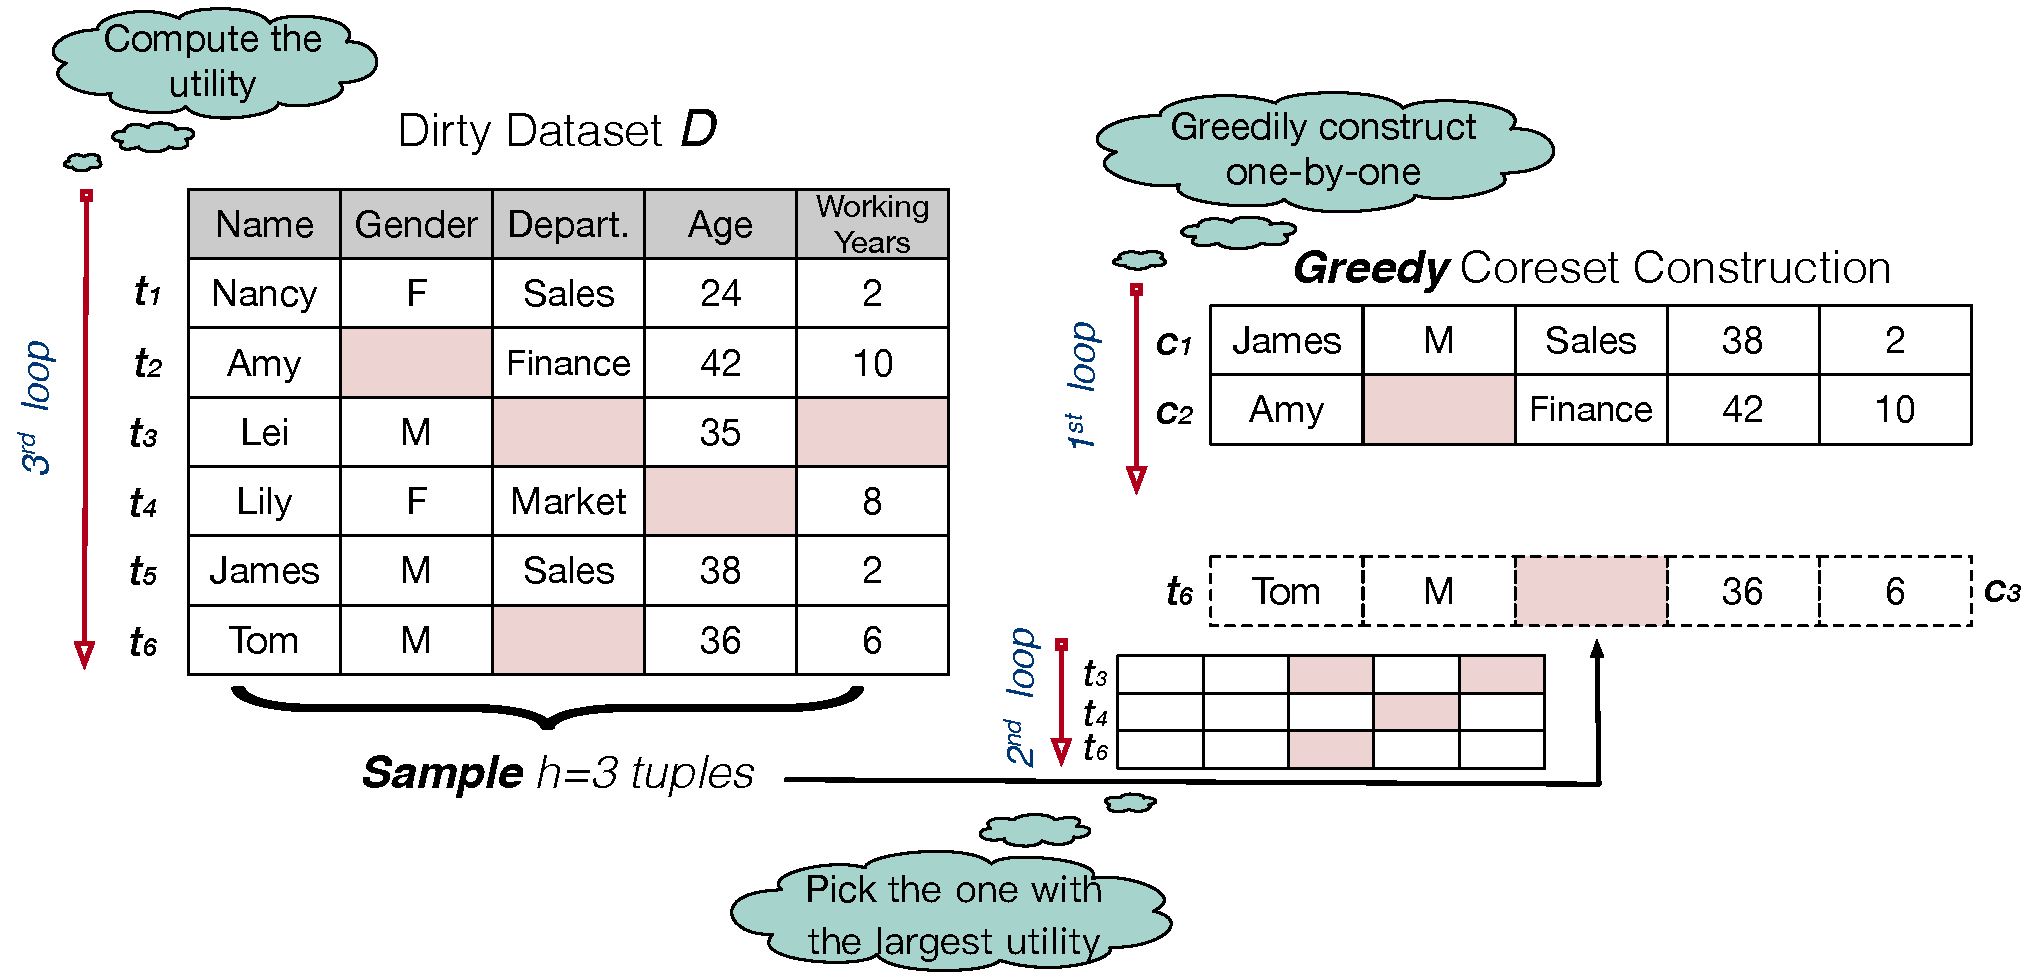
\includegraphics[width=0.6\textwidth]{figs/Overview}
%	\vspace{-2.5em}
	\caption{The \ours framework.}
	\label{fig:overview}
%	\vspace{-2em}
\end{figure}


Next, we will introduce our proposed \ours framework   to solve  Eq.~\ref{eqa:expectation}, which  is non-trivial because it  is NP-hard.
But fortunately, we prove that it has the sub-modular property (see Section~\ref{sec:without}). Hence, \ours uses a greedy framework with three loops to solve the problem with an approximate ratio. 

At a high level, the greedy strategy adds one tuple with the largest ``utility'' to the coreset iteratively, which can be considered as the first loop. In each iteration, we have to iterate tuples in $\train$ to select the one with the largest utility, which is the second loop. Naturally, we have to compute the utility of each tuple, where all tuples in  $\train$ have to be considered, leading to the third loop.
 

Next, we will further illustrate the framework using Figure~\ref{fig:overview} and Algorithm~\ref{alg:framework}.


%!TEX root = ../main.tex

\begin{figure}[!t]
 \vspace{-1em}
	\begin{algorithm}[H]
		\normalem
	\caption{\ours Framework \label{alg:framework}}
		{\small
		\KwIn{Incomplete train data $\train$, coreset size $\numcore$, sample size $h$.}
		\KwOut{A coreset $\core \subseteq \train$, weight $\weightset=\{w_j\}$,$|\core|=|\weightset|=\numcore$.}
		
		$C=\emptyset$;\\\nllabel{alg1:init1}
		
		\While{$|\core|< \numcore$}
		{\nllabel{craig1:loop1}
			
		/*1st loop*/  \\
		
		Sample $h$ tuples as $T_{sample} \subseteq \train \setminus \core$\\\nllabel{craig1:sample}
		
			\For{each tuple $t \in T_{sample}$}  
			{\nllabel{craig1:loop2}
				
				/*2nd loop*/ \\
				
			%	}
			 $\mathrm{E}[t|\core]=\texttt{ComputeUtility}(t, C,D)$;
				 /*3rd loop*/  \\\nllabel{craig1:loop3}
			}		

			$t^*$ = $\argmax_{t\in T_{sample}}\mathrm{E}[t|\core]$ ;\\\nllabel{craig1:maxmulti}
			
			$\core = \core \cup \{t^*\}$;
			\\\nllabel{craig1:add2} 
			
				%\If{$\mathbb{I}[t^*] = 1$}
		%	{ \nllabel{alg:if}
		%		 \cc{Impute $t^*$ (by human or automatic methods).}\\\nllabel{alg:oracle}
		%	
			%}					
		}

	
	    \For{ $t\in \core$} 
	    {\nllabel{craig1:goodcore1}
	       \If{$\mathbb{I}[t] = 1$} {\nllabel{craig1:oracle1}
	         Impute $t$ by a  human or automatic method.\\\nllabel{craig1:oracle}
             }
        }
	 	\For{$j = 1$ to $|\core|$} 
	 	{\nllabel{craig1:cc0}
	 		%$w_j = \sum_{i=1}^{n}\mathbb{I}'[j=\argmin_{c_{j'}\in\core}  %\max\limits_{\hypo\in\vartheta}\lVert \df_i(\hypo) - \df_{\gamma(j')}(\hypo) \rVert ]$;\\\nllabel{craig1:cc}
	 		\For{$i = 1$ to n}
	 		{
	 		  \If{$c_j=\argmin_{c_{j'}\in\core}\max\limits_{\hypo\in\vartheta}\lVert \df_i(\hypo) - \df_{\gamma(j')}(\hypo) \rVert$}
	 		  {
	 		  	$w_j~+\!=~1$;\\\nllabel{craig1:cc}
	 		  }
 		    }
	 		
	 	}
		\Return $\core,\weightset$;\\\nllabel{craig1:return}
		}
	\end{algorithm}
\end{figure}


\stitle{The first loop (lines~\ref{craig1:loop1}-\ref{craig1:add2})} of  the greedy algorithm is  to add the  tuple $t^*$ with the maximum \textit{utility} (\ie $\mathrm{E}[t|\core] = \mathrm{E}[\core] - \mathrm{E}[\core \cup \{t\}]$) into the coreset iteratively for $\numcore$ times. To be specific, the  ``utility''  of a tuple $t$ denotes the reduction of  expectation of GA error after adding $t$  into the coreset $\core$. 

Suppose that $\numcore=3$. Figure~\ref{fig:overview} (the $1^{st}$ loop part) shows the situation that there already have been 2 tuples in $\core$, and we are going to add the third tuple into the coreset.


\stitle{The second loop (lines~\ref{craig1:loop2}-\ref{craig1:loop3})} computes the utilities of  tuples  that are not in coreset $C$, based on which the best one is picked for the first loop. An ideal solution is to consider all tuples in $\train \setminus \core$, which is prohibitively expensive, so in practice we use an efficient method to accelerate
this loop by uniformly sampling $h$ tuples as $T_{sample}$ (line~\ref{craig1:sample}) and then selecting the best one from $T_{sample}$ (line~\ref{craig1:maxmulti}). The  difference is that theoretically, considering all tuples has an approximate ratio 1-$\frac{1}{e}$ (because of the sub-modular property), while the sampling method holds a (1-$\frac{1}{e}-\epsilon$) ratio~\cite{mirzasoleiman2015lazier}, where $\epsilon$ is related to the sampling ratio.

As shown in Figure~\ref{fig:overview}, suppose that $h=3$, and we sample $\{t_3, t_4, t_6\}$ from $\{t_1, t_3, t_4, t_6\}$. Then the second loop iterates the three tuples and computes the utility for each one (the third loop).


\stitle{The third loop (line~\ref{craig1:loop3})} will loop through all tuples in $\train$, so as to compute the utility of tuple $t$ used in the second loop.  To be specific, the core part of the utility computation (\ie \texttt{ComputeUtility}) is to compute $\mathrm{E}[C] = \sum_{k= 1}^{|\worlds|} p_kS_k= \sum_{k= 1}^{|\worlds|} p_k (\sum_{i=1}^n \min_{c_j\in C_k}\dist_{ij})$, from which we can see that it is inevitable to iterate the $n$ tuples in $\train$. However, the most challenging part is that we also have to enumerate a large number of possible worlds. We will illustrate how to solve this in details in Section~\ref{sec:without}.



\stitle{The imputation step (line~\ref{craig1:oracle}).} After \ours selects the coreset $C$ using the above 3 loops, we can leverage a human or automatic method to impute the tuples that are incomplete in $C$, which correspond to Case (5) and Case (6) in Section~\ref{sec:intro} respectively. 




\stitle{Weights computation (lines~\ref{craig1:cc0}-\ref{craig1:cc}).} It computes the weight of each tuple in $C$, which will be used to approximate the full gradient during training. For training, tuples in the coreset are randomly shuffled. Afterwards, suppose that in each step of the gradient decent, when we use $c_j \in \core$ to update the gradient, we compute the gradient $(\df_j)$ of $c_j$ first, and then use $w_j\df_j$ to update the model parameters. $w_j$ is the number of tuples in $\train$ assigned to $c_j$.  The above steps repeat until the model converges.


\stitle{Optimizations of imputation-in-the-loop.} Unfortunately, the 3-loop computation of the strategy is rather expensive due to the large number of possible worlds (Section~\ref{sec:without}).   To address this, we can   integrate either human-in-the-loop or the automatic method into \ours framework (Section~\ref{sec:human}).  It iteratively imputes one incomplete tuple or a mini-batch of incomplete tuples. Once the tuple(s) is (are) computed and added to the coreset within the first loop, the number of possible worlds can be significantly reduced, and so does the computational cost. %In addition, how to select an appropriate coreset size $K$ is an important problem, which will be discussed in Section~\ref{exp:sec:end2end}.

%\cc{Do we need to say why this optimization can solve the complexity? But easy to be redundant with Sec 5}

%The advantages of the optimization are two-fold. First, with more and more missing values are imputed, the number of possible worlds are greatly reduced, which reduces the machine cost a lot. Second, for human imputation, it allows us to  gradually impute the tuples accurately, and thus the coreset score computation can be more and more accurate, which produces a better coreset.

\stitle{Group-based acceleration.} \cc{As discussed above, we have to iterate all tuples of $D$ in the third loop to compute the utility of a tuple $t$. Given a large train set with missing values, it is still inefficient to compute the coreset. To address this, we propose to assign tuples in $D$ to multiple groups, and use these groups to represent the entire dataset. Since the number of groups are smaller than $n$, the efficiency can be much improved (Section~\ref{sec:group}).}  














